% -*- mode: fundamental -*-

% ================================================================

\begin{frame}[fragile]
\frametitle{Reminders}

\footnotesize

Please git clone or git pull: \url{https://github.com/rsnikhil/Learn_Bluespec_and_RISCV_Design}

\begin{Verbatim}[frame=single, numbers=left]
    ./Book_BLang_RISCV.pdf
      Slides/
          Slides_01_Intro.pdf
          Slides_02_ISA.pdf
          ...
      Doc/Installing_bsc_Verilator_etc.{adoc,html}
      Exercises/
          Ex_03_B_Top_and_DUT/
          Ex_03_A_Hello_World/
          ...
      Code/
          src_Common/
          src_Drum/
          src_Fife/
          src_Top/
          ...
\end{Verbatim}

\vspace{1ex}

To compile and run the code for exercises, Drum and Fife, please make sure you have installed:

\begin{itemize}

 \item \emph{bsc} compiler (see \url{https://github.com/B-Lang-org/bsc})

 \item Verilator compiler (see \url{https://www.verilator.org/})
\end{itemize}

\footnotesize

\end{frame}

% ================================================================

\begin{frame}
\frametitle{Chapter Roadmap}

\footnotesize

\begin{center}
\frame{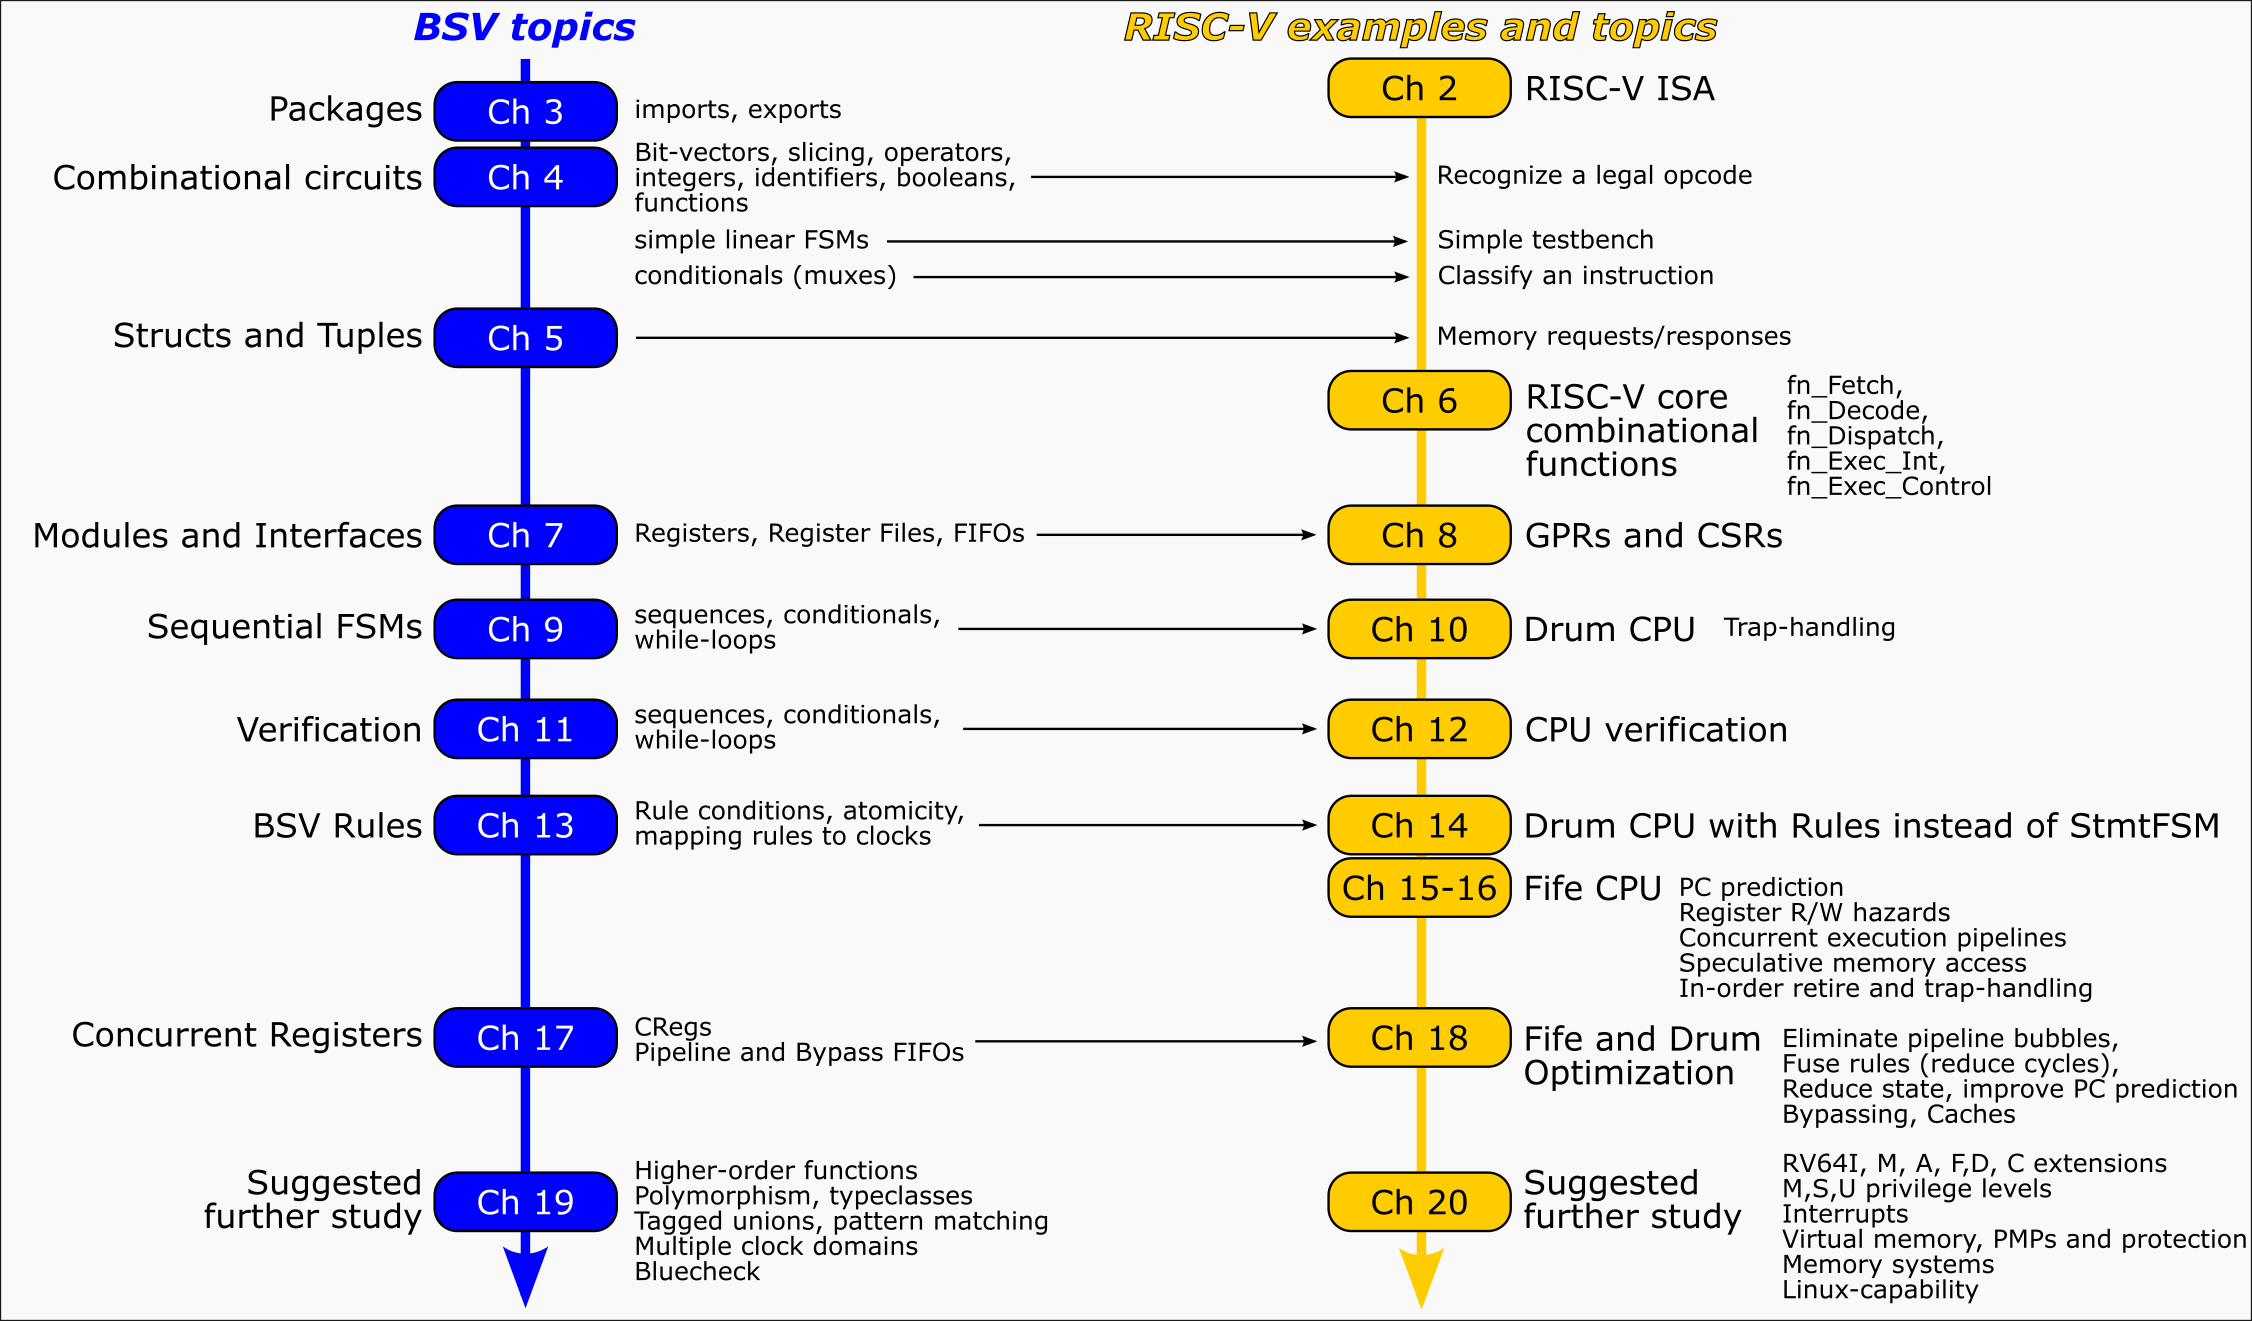
\includegraphics[height=0.825\textheight]{Fig_Chapter_Roadmap}}
\end{center}

\end{frame}

% ================================================================
